\documentclass{sigchi}

\toappear{CS3301: Component Technology Practical 1: Middleware}

\pagenumbering{arabic}

\usepackage{balance} 
\usepackage{graphics}
\usepackage{times}
\usepackage{url}
\usepackage{amsmath}
\newcommand{\BigO}[1]{\ensuremath{\operatorname{O}\bigl(#1\bigr)}}

\makeatletter
\def\url@leostyle{%
  \@ifundefined{selectfont}{\def\UrlFont{\sf}}{\def\UrlFont{\small\bf\ttfamily}}}
\makeatother
\urlstyle{leo}

\def\pprw{8.5in}
\def\pprh{11in}
\special{papersize=\pprw,\pprh}
\setlength{\paperwidth}{\pprw}
\setlength{\paperheight}{\pprh}
\setlength{\pdfpagewidth}{\pprw}
\setlength{\pdfpageheight}{\pprh}

\usepackage[pdftex]{hyperref}
\hypersetup{
pdftitle={SIGCHI Conference Proceedings Format},
pdfauthor={LaTeX},
pdfkeywords={SIGCHI, proceedings, archival format},
bookmarksnumbered,
pdfstartview={FitH},
colorlinks,
citecolor=black,
filecolor=black,
linkcolor=black,
urlcolor=black,
breaklinks=true,
}
\providecommand*{\lstnumberautorefname}{line} 
\newcommand\tabhead[1]{\small\textbf{#1}}

\usepackage{color}
\usepackage{upquote}
\usepackage{listings}
\lstset{ %
upquote=true
basicstyle=\footnotesize,       % the size of the fonts that are used for the code
numbers=left,                   % where to put the line-numbers
numberstyle=\footnotesize,      % the size of the fonts that are used for the line-numbers
stepnumber=1,                   % the step between two line-numbers. If it is 1 each line will be numbered
numbersep=5pt,                  % how far the line-numbers are from the code
backgroundcolor=\color{white},  % choose the background color. You must add \usepackage{color}
showspaces=false,               % show spaces adding particular underscores
showstringspaces=false,         % underline spaces within strings
showtabs=false,                 % show tabs within strings adding particular underscores
frame=single,           % adds a frame around the code
tabsize=2,          % sets default tabsize to 2 spaces
captionpos=b,           % sets the caption-position to bottom
breaklines=true,        % sets automatic line breaking
breakatwhitespace=false,    % sets if automatic breaks should only happen at whitespace
escapeinside={\%*}{*)}          % if you want to add a comment within your code
}
\renewcommand\lstlistingname{Code Fragment}

\usepackage[english]{babel}
\usepackage[autostyle]{csquotes}

\begin{document}

\title{Component Tech: TopHat, A Middleware for Sensor Data}

\numberofauthors{2}
\author{
  \alignauthor 110011264\\
    \affaddr{School of Computer Science}\\
    \affaddr{University of St Andrews}\\
  \alignauthor 110002255\\
    \affaddr{School of Computer Science}\\
    \affaddr{University of St Andrews}\\
}

\maketitle

\begin{abstract}
The report describes the design, implementation, and evaluation of TopHat, a message oriented middleware that handles the transmission of mobile sensor data. The concepts of producers and consumers are used. The load balancer behind the middleware is also discussed.
\end{abstract}

\section{REPORT}

\subsection{Planning}

Initially, the team implemented a simple server. The server receives heartbeats, in the form of POST request, from the producers. Each heartbeat consisted of an unique identifier of the mobile phone device and its current location. The sender advertises itself as a producer to the server. When a consumer asks the server for sensor data from that particular producer, the server will send a request to the producer, and then pass on the results back to the producer. However, this approach requires the producers listening on some ports to handle data requests from the server. As a result, the consumer will spend significant time waiting for the server to retrieve data from the producer. The solution will create too much overhead on the server side, and it is unlikely that the server can deal with increasing consumer requests.

Later on, the team arrived to a more elegant solution. On each heartbeat, the producer sends sensor data to the server. The server caches the data, and flushes them to a persistent database on occasion. Now, when a consumer requests sensor data from a particular producer, the server can respond quickly, since the sensor data are cached. A more detailed description of the overall setup is explained in the next section.

\subsection{Instructions}

See \enquote{README.md} in the project directory for directions on how to run the servers, producers, and consumers. The file describes the arguments needed to run each system component.

\subsection{Design}

\subsubsection{System components}

The final system architecture at the time of our submission consists of:

\begin{itemize}
  \item 1 Load balancer
  \item N Workers
  \item X Producers
  \item Y Consumers
\end{itemize}

\begin{figure}[!h]
\centering
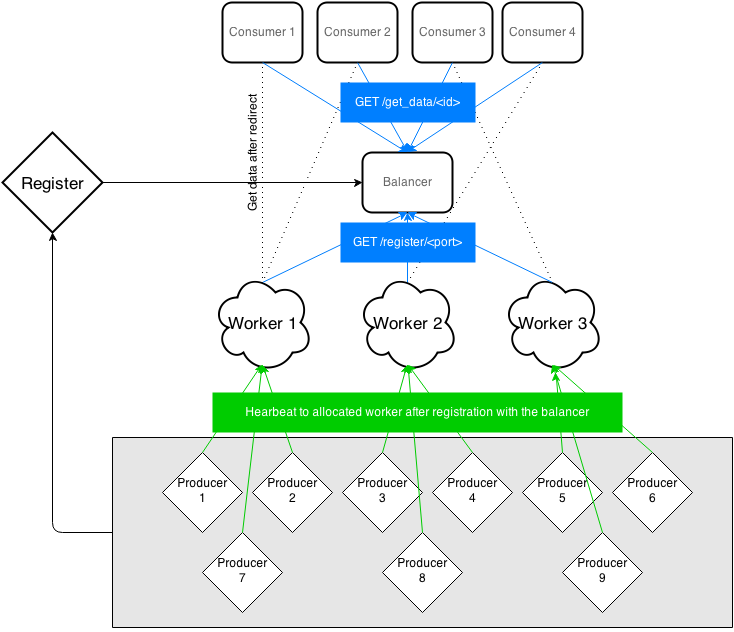
\includegraphics[width=0.9\columnwidth]{img/main}
\caption{The final system architecture}
\label{fig:main}
\end{figure}

A load balancer is the primary component of the system. It manages every other system component and balances the server load. A worker is a separate unit that is responsible for data retrieval and storage. A producer generates sensor data, and a consumer requests those data. An example of a producer would be a mobile phone, and an example of a consumer would be a web service that uses location data to recommend music to its users.

\subsubsection{Load balancer and workers}

The load balancer is the entry point of the entire system. It is initialised to be listening on a specified port. It supports a number of RESTful API calls that allows other entities to interact with its system components, such as a worker. The worker is initialised with the IP address and the port number of the load balancer, so that it can register itself as a worker for the load balancer via with the {\it /balancer/int:port} API call. The load balancer processes the registration request, and stores the worker's IP address in memory. The load balancer keeps track of every worker, and will distribute the server load evenly, using the round robin method. Every worker must go through the above registration process in order to let itself known to the load balancer, whom will redirect producers and consumers to the worker. The worker also listens on a specified port, for handling heartbeats (described below) and sensor data requests. It is worth noting that the worker will exit if it cannot connect to the load balancer.

\begin{figure}[!h]
\centering
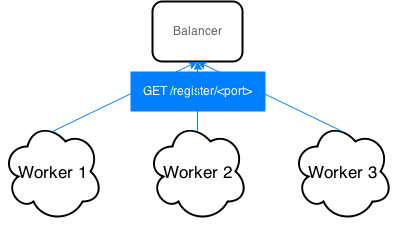
\includegraphics[width=0.9\columnwidth]{img/workerreg}
\caption{Workers need to register with the balancer before they can start accepting work.}
\label{fig:worker}
\end{figure}

\subsubsection{Load balancer and producers}

Producers ask the load balancer to be assigned with a worker. Afterwards, the producers only communicate with their assigned workers, and only when the connection disconnects do they speak to the load balancer again. To register, the producers fire the {\it /register/int:id} API call to the load balancer, with its ID. The producer ID is the unique identifier of the mobile device, also known as the International Mobile Station Equipment Identity, or IMEI. After registration, the load balancer returns the IP address of an available worker to the producer. The load balancer keeps track of the mapping between producers and workers. When a consumer requests data from a certain producer, the load balancer will redirect the request to the worker that has been in contact with that producer. HTTP errors such as disconnected connection and interruption are caught and handled.

\begin{figure}[!h]
\centering
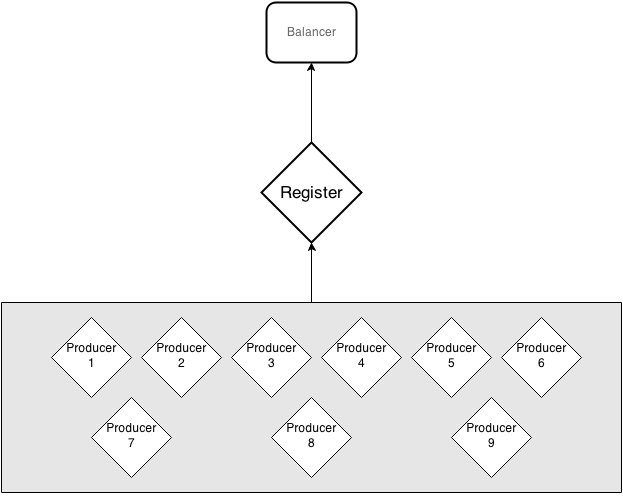
\includegraphics[width=0.9\columnwidth]{img/producer}
\caption{A producer first registers with the balancer and is assigned a worker}
\label{fig:producer}
\end{figure}

\subsubsection{Workers and producers: heartbeats}

After a producer receives its assigned worker and the corresponding IP address, it will continuously send heartbeats (periodic messages) to that worker. The message contains the following information:

\vspace*{\baselineskip}
\begin{lstlisting}[caption={Heartbeat format}, mathescape, upquote=true]
received_heartbeat = {
  'id': id
  'location': location
  'data': data
}

new_heartbeat = {
  'id': int(request.json['id']),
  'location': request.json['location'],
  'ip_address': request.remote_addr,
  'timestamp': datetime.utcnow(),
  'data': request.json['data']
}
\end{lstlisting}

On each heartbeat POST request, the worker extracts the \enquote{id}, \enquote{location}, and \enquote{data} from \enquote{received\_heartbeat}. In addition, the worker takes note of the remote IP address of the request, as well as the current time. The worker puts the information altogether into a new \enquote{heartbeat} object called \enquote{new\_heartbeat} (a dictionary in $Python$). The team has designed a data structure called cache, defined in $worker/cache.py$. In essence, the cache stores a mapping (another dictionary) between the producer ID and the its latest \enquote{heartbeat}. The worker will flush the \enquote{heartbeats} to the database every $20$ seconds. The time interval is chosen for demonstration purposes, and more tests are needed to find out the optimal time. The worker will also flush the cache to the database when it reaches the size limit. The size is kept to $100$, also for demonstration purposes. When the cache is full and the contained data are added to the database, half of the cache is cleared to allow more data to be added.

If the worker goes offline or crashes, the producer will ask for a new worker from the load balancer. The producer will do so for a specified number of times (10 in the current system), until it gets a new worker or uses all of the attempts. The number is chosen for no particular reason, and further experiments are required to find the optimal value. The number of retries can also be specified by the user and it can be indefinite, meaning that the producer will always be waiting for an available worker. When the producer gets a new worker, it will resume sending heartbeats. All errors regarding connection loss and interruption are handled.

\begin{figure}[!h]
\centering
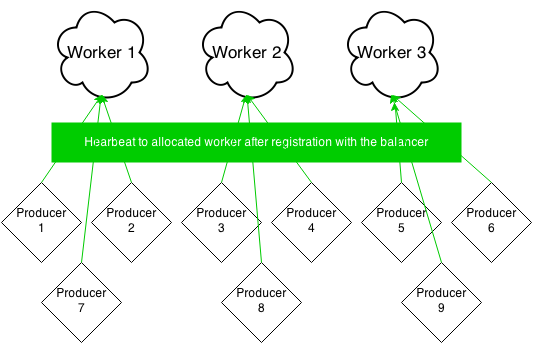
\includegraphics[width=0.9\columnwidth]{img/heartbeat}
\caption{Producers send heartbeats to their assigned workers.}
\label{fig:heartbeat}
\end{figure}

\subsubsection{Load balancer and consumers: redirection}

A consumer requests data through the load balancer. As mentioned above, the load balancer keeps track of the relationship between producers and workers. It redirects the consumer to the appropriate worker, where the data are received and stored in real time.

The following scenario describes a typical use case. A consumer makes the {\it /get\_data/int:id} API call to the load balancer. The load balancer checks whether the producer ID is being handled by anyone of the workers. If so, the consumer will be redirected to the appropriate worker. The worker will handle the request and return the data that the consumer asks for. All connection errors that might occur are handled and do not cause crashes.

\begin{figure}[!h]
\centering
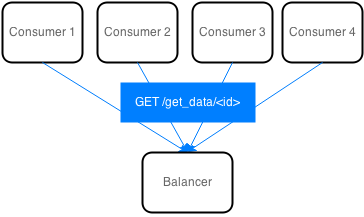
\includegraphics[width=0.9\columnwidth]{img/consumer_req}
\caption{Consumers request data from the load balancer}
\label{fig:consumer_req}
\end{figure}

\subsubsection{Workers and consumers}

The worker does several things after being contacted by a redirected consumer (See Figure \ref{fig:cons_to_worker}). Firstly, it checks whether it has the data in the cache. If so, the worker will return the data to the consumer. Otherwise, the worker will issue a database query to find such data from the database. The cache greatly reduces the number of database queries, while improving response times.

\begin{figure}[!h]
\centering
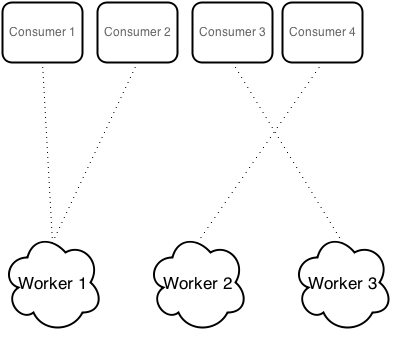
\includegraphics[width=0.9\columnwidth]{img/cons_to_worker}
\caption{Workers and consumers relationships}
\label{fig:cons_to_worker}
\end{figure}

\subsubsection{Why Flask?}

The team decides to use the python web framework Flask, alongside with Requests and SQLite. SQLAlchemy is used to manage and migrate the database with ease. There is no particular reason to use SQLite over other existing databases. A SQLite database is sufficient for the extent of this practical, and there has been no discussion on the optimisation of the database. The python web framework Tornado is also used to help scale the system. It easily integrates with Flask and scales extremely well, which means it is ideal for real-time web services.

\subsubsection{Why RESTful?}

A decision was made to base the system on a RESTful API. RESTful API provide a simple standardized communication over HTTP, which is stateless. Also, the technology is very convenient to use on mobile devices. The language that was chosen was Python and bash for the shell scripts used to simulate and test the system. 

\subsection{Testing}

The team has included a number of simple tests cases inside the $tests$ directory. See \enquote{README.md} on instructions of how to run them. Make sure the system has all the listed dependencies. There are two extra tests below that examine the time taken for requests, in relation to the number of workers available.

\subsubsection{Timing Test 1: Load balancer}

Setup:

\begin{itemize}
  \item 1 Load balancer
  \item 3 Workers
  \item 20 Producers
  \item 5 Consumers scripts
\end{itemize}

\vspace*{\baselineskip}
\begin{lstlisting}[caption={Timing test 1: instructions}, mathescape, upquote=true]
On one machine:
  python run_balancer 5000
  python run_worker 6000 localhost 5000
  python run_worker 6001 localhost 5000
  python run_worker 6002 localhost 5000

On a different machine:
  ./run_producers.sh balancer_addr balancer_port 3000 20
  ./run_consumers.sh balancer_addr balancer_port 3000 20
\end{lstlisting}

The time per request with all workers running is ~0.02 seconds, whereas the time per request with only one worker running increases to ~0.06 seconds. This test demonstrates that when the load balancer distributes the server load to a number of workers, it reduces the response time per request on the consumer side. It also reduces the resource load, for example memory, for each worker.

\subsubsection{Timing Test 2: Concurrent connection}

The setup is similar to that of the previous timing tests, with the addition of ab, an Apache HTTP server benchmarking tool. The tool sends a number of concurrent requests to the server. We use this tool to examine whether the server displays any unexpected behaviour when the number of requests increases dramatically.

\begin{itemize}
  \item 1 Load balancer
  \item 3 Workers
  \item 20 Producers
  \item 10 Consumers scripts
  \item Apache ab benchmark tool
\end{itemize}

Instructions:

\vspace*{\baselineskip}
\begin{lstlisting}[caption={Apache ab testing: instruction}, mathescape, upquote=true]
  ab -n 3000 -c 500 <balancer_addr>:<balancer_port>/get_data/<producer_id>
\end{lstlisting}

The time per request is 3.86 ms across all concurrent requests. The server handles the load gracefully when multiple concurrent requests are made.

\subsection{Evaluation and Conclusion}

The system is fault-tolerant and scalable. If we were to have more resources, we would deploy the service onto a an actual web server, or a web instance, and analyze how the current implementation scales. We did not have time to make a dynamic load balancer, which would distributes the load based on the number of requests a particular worker had received.

\subsection{Extra: How we collaborated}

The team composed of two people, and both members had coding sessions in the lab on a daily basis. The work was divided evenly, and usually the members would decide among themselves which parts of the practical they wanted to work on a particular day. In general, one worked on the servers, cache, and database, and the other worked on the producers, consumers, and the load balancer. The team did testings together, either on local machines and on several machines, and one of us made test scripts (those in the \enquote{tests} directory) that captured more or less our tests.

The team approached the task by making a minimum viable product at first, then improving it with incremental changes. The team aimed to meet the specification, with well-documented and structured code. In the end, both members agreed that they had meet the goal and had a productive experience.

\end{document}
